
\documentclass[preprint,12pt]{elsarticle}

\usepackage[spanish]{babel}
\usepackage{amssymb}
\usepackage{graphicx}
\usepackage{lineno}
\usepackage[utf8]{inputenc}
\usepackage{url}
\usepackage{natbib} 
\usepackage{amsmath} 
\usepackage{amssymb} 
\usepackage{float}

\begin{document}
	
	\begin{frontmatter} 

		\title{\huge INFORME DE LABORATORIO 08 INSTALACION DE UN GESTOR DE BASE DE DATOS ORACLE}
		
		\author{Huichi Contreras, Franklin Carlos         	(2016054948)} 
		\address{Escuela Profesional de Ingeniería de Sistemas}
		\address{Universidad Privada de Tacna}
		\address{Tacna, Perú}
		

	\end{frontmatter}

%% INTRODUCION ----------------------------------------------------------------------------------------------------------------

\section{INFORMACIÓN GENERAL} 

\subsection {\textbf{Objetivos}}
\begin{itemize}
	\item Instalación de de un Gestor de Base de Datos Oracle
\end{itemize}

\subsection {\textbf{Equipos, materiales, programas y recursos utilizados}}
\begin{itemize}
	\item Computadora con sistema operativo Windows XP, Vista, Windows 7, Windows 8 y/o Windows 8.1.
	\item CPU SLAT-capable feature al menos 4GB de RAM
	\item Docker Desktop (Para lo cual se debe primero crear una cuenta en Docker Hub)
	\item Oracle SQL Developer for Windows 
\end{itemize}

%% ----------------------------------------------------------------------------------------------------------------------------------


%% MARCO TEÓRICO ------------------------------------------------------------------------------------------------------------

\section{Marco Teórico}

%% PRIMERA SUBSECCION 

\subsection {\textbf{Docker}}
Docker se define como un proyecto de código abierto que proporciona una capa de abstracción y virtualización a nivel de sistema operativo, a través de la instalación de contenedores de software.
\subsubsection{\textbf{SQL Server Management Studio}}
Oracle SQL Developer 64 bits es un entorno de desarrollo integrado y gratuito que simplifica el desarrollo y la administración de Oracle Database tanto en implementaciones tradicionales como en la nube.


\section{PROCEDIMIENTO}

\subsubsection{\textbf{Paso 1: Gestionar Docker Setup}}
\begin{figure}[H]
	\begin{center}
		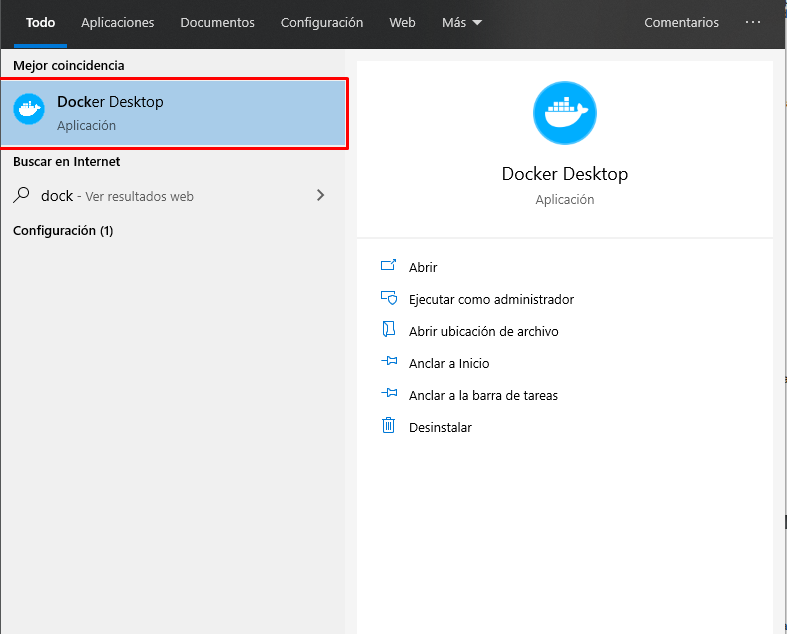
\includegraphics[width=12cm]{./IMAGENES/foto1} 
		\caption{Ingresar a Docker Setup}
	\end{center}
\end{figure}

\begin{figure}[H]
	\begin{center}
		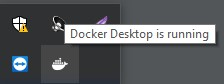
\includegraphics[width=12cm]{./IMAGENES/foto2} 
		\caption{Comprobamos que esta arrancando el Docker}
	\end{center}
\end{figure}

\begin{figure}[H]
	\begin{center}
		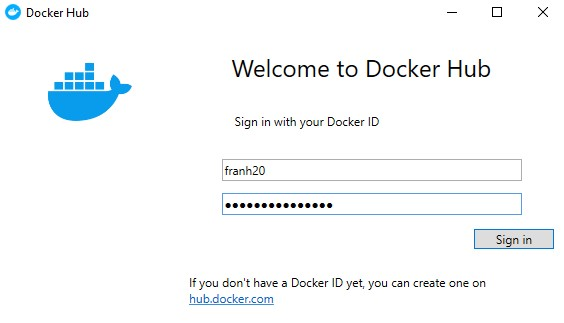
\includegraphics[width=12cm]{./IMAGENES/foto3} 
		\caption{Ingresamos nuestra cuenta de Docker}
	\end{center}
\end{figure}

\begin{figure}[H]
	\begin{center}
		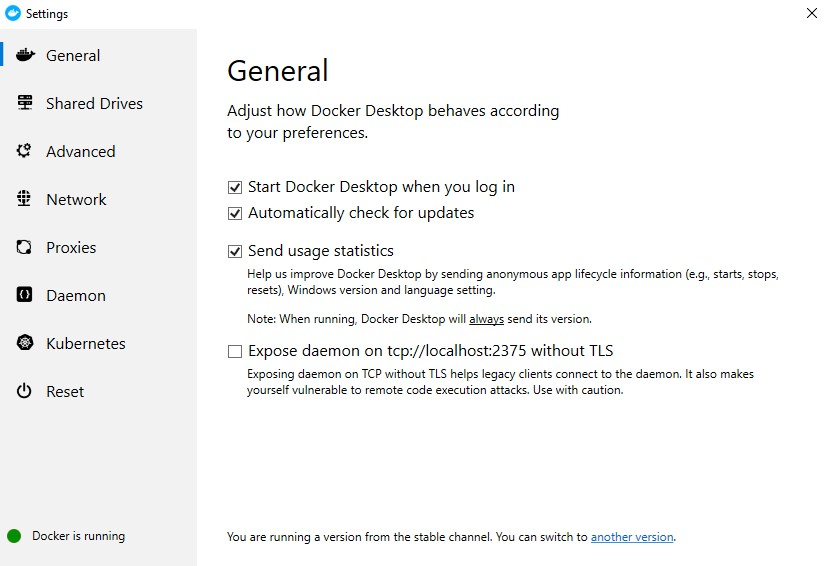
\includegraphics[width=12cm]{./IMAGENES/foto4} 
		\caption{Como se ve podemos ver los ajustes del Docker.}
	\end{center}
\end{figure}

\subsubsection{\textbf{Paso 2: Gestionar los contenedores mediante PowerShell}}

\begin{figure}[H]
	\begin{center}
		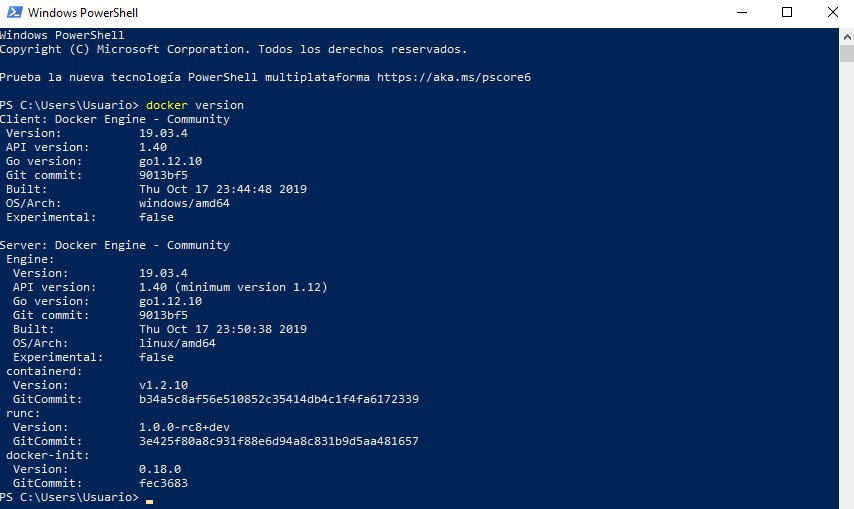
\includegraphics[width=12cm]{./IMAGENES/foto5} 
		\caption{Ingresamos “Docker versión” para ver si tenemos Docker}
	\end{center}
\end{figure}


\begin{figure}[H]
	\begin{center}
		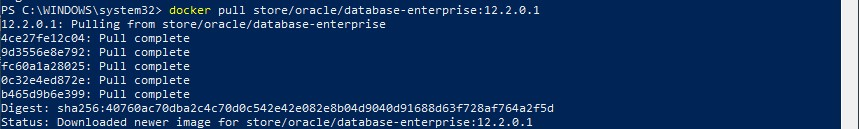
\includegraphics[width=12cm]{./IMAGENES/foto6} 
		\caption{Descargamos la iso definidar}
	\end{center}
\end{figure}

\begin{figure}[H]
	\begin{center}
		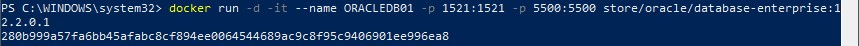
\includegraphics[width=12cm]{./IMAGENES/foto10} 
		\caption{Instalamos nuestro contenedor}
	\end{center}
\end{figure}

\begin{figure}[H]
	\begin{center}
		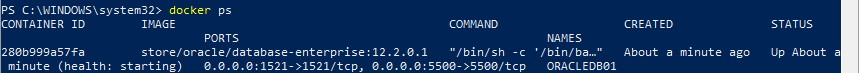
\includegraphics[width=12cm]{./IMAGENES/foto11} 
		\caption{Verificamos que tenemos instalado}
	\end{center}
\end{figure}

\subsubsection{\textbf{Paso 3: Ejecutar}}
\begin{figure}[H]
	\begin{center}
		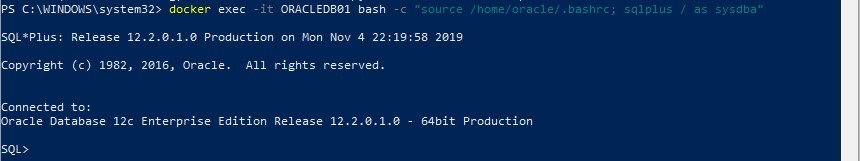
\includegraphics[width=12cm]{./IMAGENES/foto12} 
		\caption{Ejecutamos el docker}
	\end{center}
\end{figure}

\begin{figure}[H]
	\begin{center}
		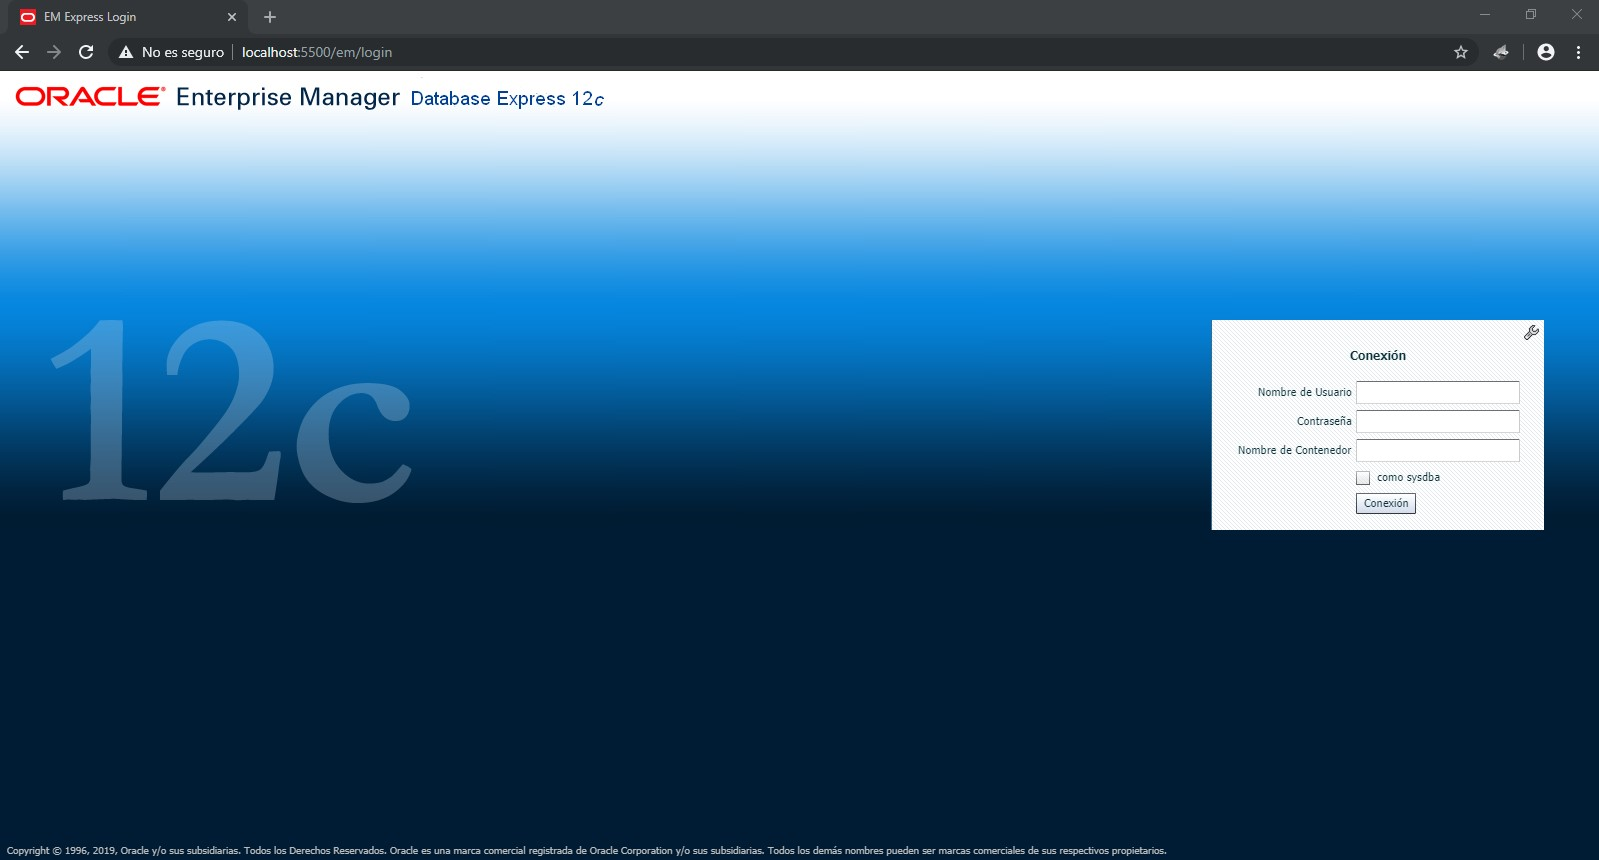
\includegraphics[width=12cm]{./IMAGENES/foto13} 
		\caption{Conectadonos a la base de datos creadas}
	\end{center}
\end{figure}

\begin{figure}[H]
	\begin{center}
		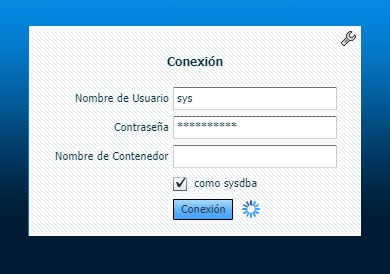
\includegraphics[width=12cm]{./IMAGENES/foto14} 
		\caption{Conectadonos a la base de datos creadas}
	\end{center}
\end{figure}

\begin{figure}[H]
	\begin{center}
		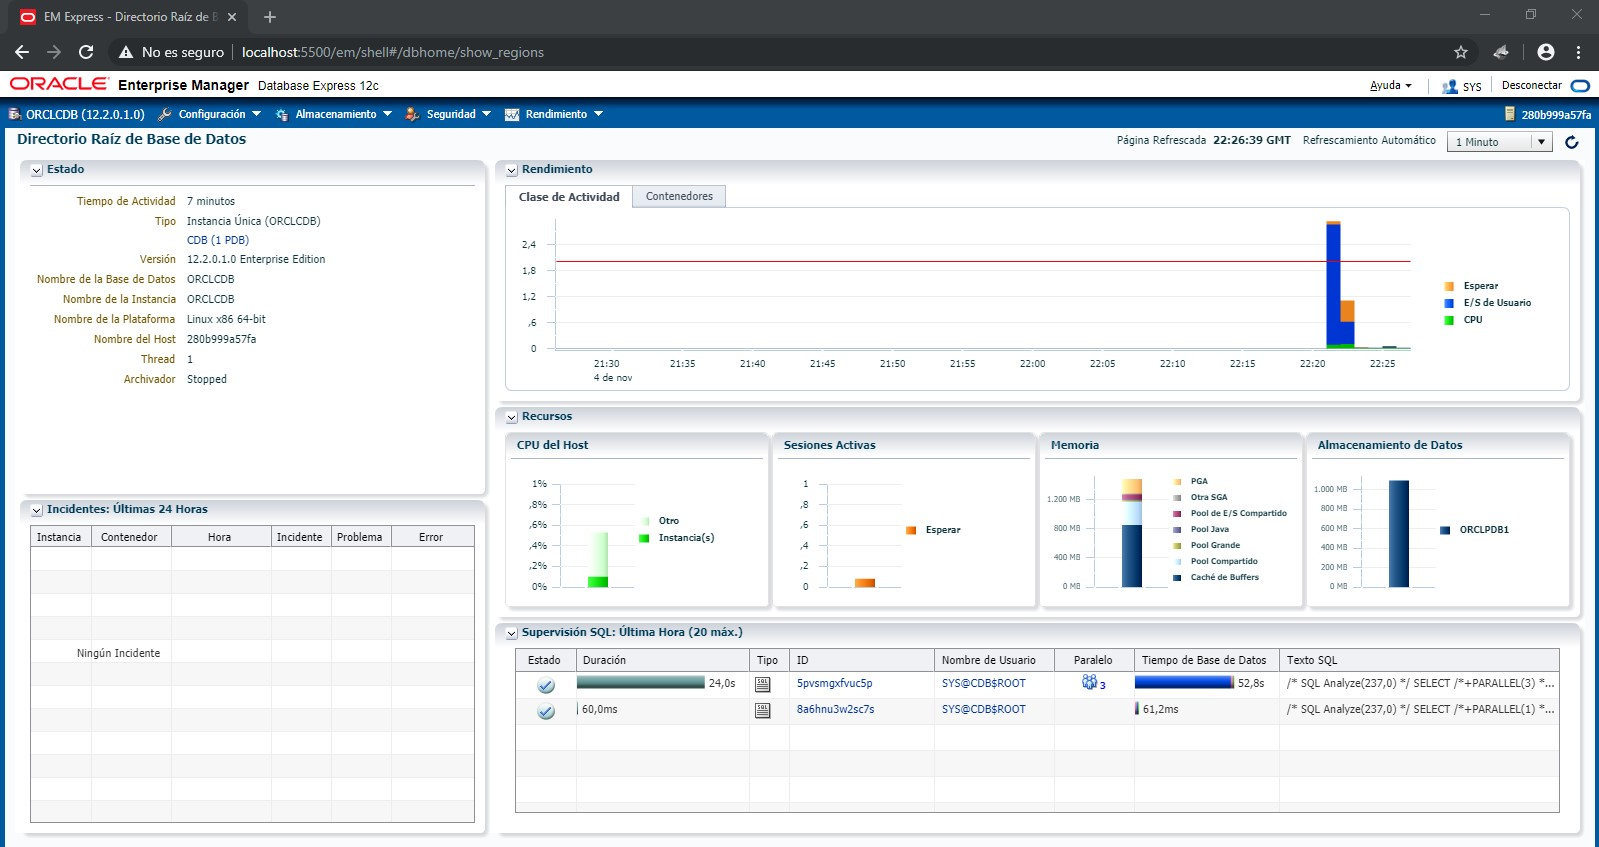
\includegraphics[width=12cm]{./IMAGENES/foto15} 
		\caption{Conectadonos a la base de datos creadas}
	\end{center}
\end{figure}

\begin{figure}[H]
	\begin{center}
		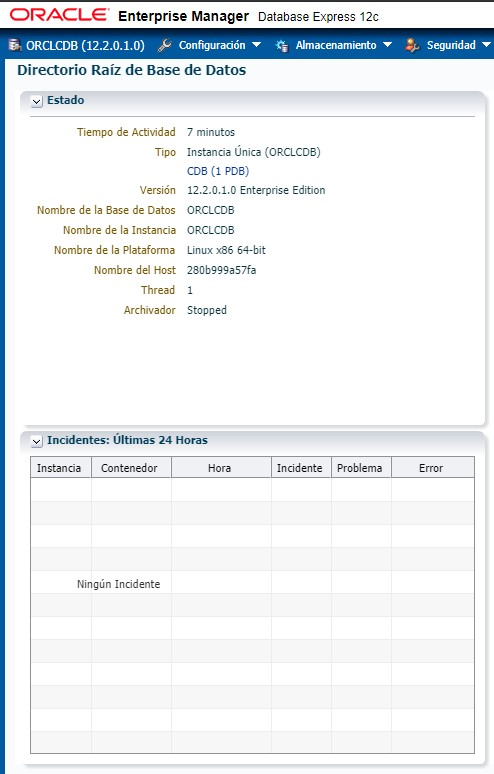
\includegraphics[width=12cm]{./IMAGENES/foto16} 
		\caption{Conectadonos a la base de datos creadas}
	\end{center}
\end{figure}

\section{ANALISIS E INTERPRETACION DE RESULTADOS }
\begin{itemize}
	\item ¿Qué indican los resultados? \\
	Pudimos realizar exitosamente la conexión de nuestro contenedor a la base de datos
	\item ¿Que se ha encontrado?\\
	Encontré una manera más rápida de poder tener una base de datos Oracler sin necesidad de estar haciendo toda la instalación necesaria en mi computadora.
\end{itemize}


\section{CONCLUSION}
En conclusión, los contenedores nos ayudan a montar nuestra base de datos de forma mas rápida para poder manejar nuestros diversos sistemas a implementarlos y conectarlos, a su vez también aprendí que los ISO nos vienen a permitir con Docker subirlas para poder usarlas en otras ocasiones.

\end{document}
